\documentclass[12pt]{report}


% ====================== PACKAGES ======================
\usepackage[french]{babel} % French language support
\usepackage[utf8]{inputenc} % UTF-8 encoding
\usepackage[T1]{fontenc} % Character encoding
\usepackage{amsmath, amssymb, amsfonts} % Math packages
\usepackage{graphicx} % Required for inserting images
\usepackage{float} % Improved handling of floating elements
\usepackage{hyperref} % For hyperlinks
\usepackage{array, tabularx, multirow, multicol} % Table packages
\usepackage{caption, subcaption} % Caption and subcaption for figures and tables
\usepackage{setspace} % Set line spacing
\usepackage{abstract} % Abstract layout
\usepackage{color, xcolor} % Color handling
\usepackage{lipsum} % For generating filler text
\usepackage{fancyhdr} % Fancy headers and footers
\usepackage{titlesec} % Section formatting
\usepackage{enumerate} % Enumerate with custom labels
\usepackage{booktabs, colortbl} % Improved table formatting
\usepackage{geometry} % To define page margins
\usepackage{longtable} % For tables spanning multiple pages
\usepackage{listings}
\usepackage{bm}

% ====================== COMMANDS ======================
\providecommand{\abs}[1]{\lvert#1\rvert} % Absolute value command
\DeclareMathOperator{\sign}{sign} % Sign function

% ====================== PAGE GEOMETRY ======================
\geometry{top=2cm, bottom=3cm, left=2cm, right=2cm} % Adjust top margin to provide space for header
\setlength{\headheight}{45pt} % Increase headheight to fit header content
\setlength{\headsep}{20pt} % Add space between header and text

% ====================== PDF METADATA ======================
\hypersetup{ % Information about the PDF document
    pdfauthor = {Premier Auteur}, % Authors
    pdftitle = {Nom du Projet - Sujet du Projet}, % Title
    pdfsubject = {Mémoire de Projet}, % Subject
    pdfkeywords = {Tag1, Tag2, Tag3}, % Keywords
    pdfstartview={FitH}, % Adjust page width to screen width
    colorlinks=true, % Colored links
    citecolor=black, % Citation links color
    filecolor=black, % File links color
    linkcolor=black, % Internal links color
    urlcolor=black % URL links color
}

\lstset{
    language=Python,
    basicstyle=\ttfamily\footnotesize,
    keywordstyle=\color{blue},
    commentstyle=\color{orange},
    stringstyle=\color{red},
    showstringspaces=false,
    numberstyle=\tiny\color{gray},
    numbers=left,
    stepnumber=1,
    numbersep=5pt,
    frame=single,
    breaklines=true,
    backgroundcolor=\color{lightgray},
    captionpos=b,
    tabsize=4,
    morekeywords={Material, self},
}

% ====================== HEADER AND FOOTER ======================
\pagestyle{fancy} % Enable fancy headers and footers
\fancyhf{} % Clear all header and footer fields

\fancyhead[L]{ % Left header
    \begin{minipage}{1.5cm}
        \centering
        
\includegraphics[width=0.80\textwidth]{imgs/LogoCN_Q.pdf}
    \end{minipage}
    \begin{minipage}{12cm}
        \small \textsc{École}\\
        \small \textsc{Centrale}\\
        \small \textsc{Nantes}\\
    \end{minipage}
}
\fancyhead[R]{ % Right header
    \begin{minipage}{4.8cm}
        \raggedleft
        \small \textsc{stage vision}\\
    \end{minipage}
}
\fancyfoot[R]{\large \textbf{\thepage}} % Right footer with page number

\renewcommand{\headrulewidth}{0.2pt} % Header rule width
\renewcommand{\footrulewidth}{0.2pt} % Footer rule width

% ====================== SECTION FORMATTING ======================
\titleformat{\chapter}[display]
    {\normalfont\bfseries}{}{0pt}{\Large}
\titlespacing*{\chapter}{0pt}{-20pt}{20pt}

% ====================== BEGIN DOCUMENT ======================
\begin{document}
\pagenumbering{arabic} % Start page numbering in arabic numerals
\renewcommand{\labelenumii}{\arabic{enumi}.\arabic{enumii}}

% Title page
\begin{titlepage}
    \centering
    \vspace*{0cm}
    
\includegraphics[width=0.3\textwidth]{imgs/LogoCN_Q.pdf}
    
    \vspace{3cm}
    
    \Huge\textbf{Rapport TP2 : ACSIP}\\
    \vspace{1cm}
    \Large\textbf{Perceptions}\\
    
    \vspace{2cm}
    \Large\textbf{Exercice de design : Resynthèse d’un cri d’oiseau }\\
    
    \vfill
    
    \Large{Auteur : Viozelange Matis}\\
    \vspace{0.5cm}
    
    \vfill

    \vspace{2cm}
    
    \Large\textit{date :}\\
    \Large\textit{}{17/09/2024}\\
    
    \vspace{0.5cm}
    
    \Large\textbf{École Centrale Nantes}\\
    
    \vspace*{1cm}
\end{titlepage}


\newpage
\thispagestyle{empty}
~

\chapter{Synthèse du cri de l'aigle}

Pour synthétiser le cri de l'aigle, nous proccédons tout d'abord à l'analyse du signal sonore. %
On obtient les figure \ref{fig:eaglesignaltemp}, \ref{fig:eaglespectrefreq} et \ref{fig:eaglespectrogramme}.

\begin{figure}[htbp]
    \centering
    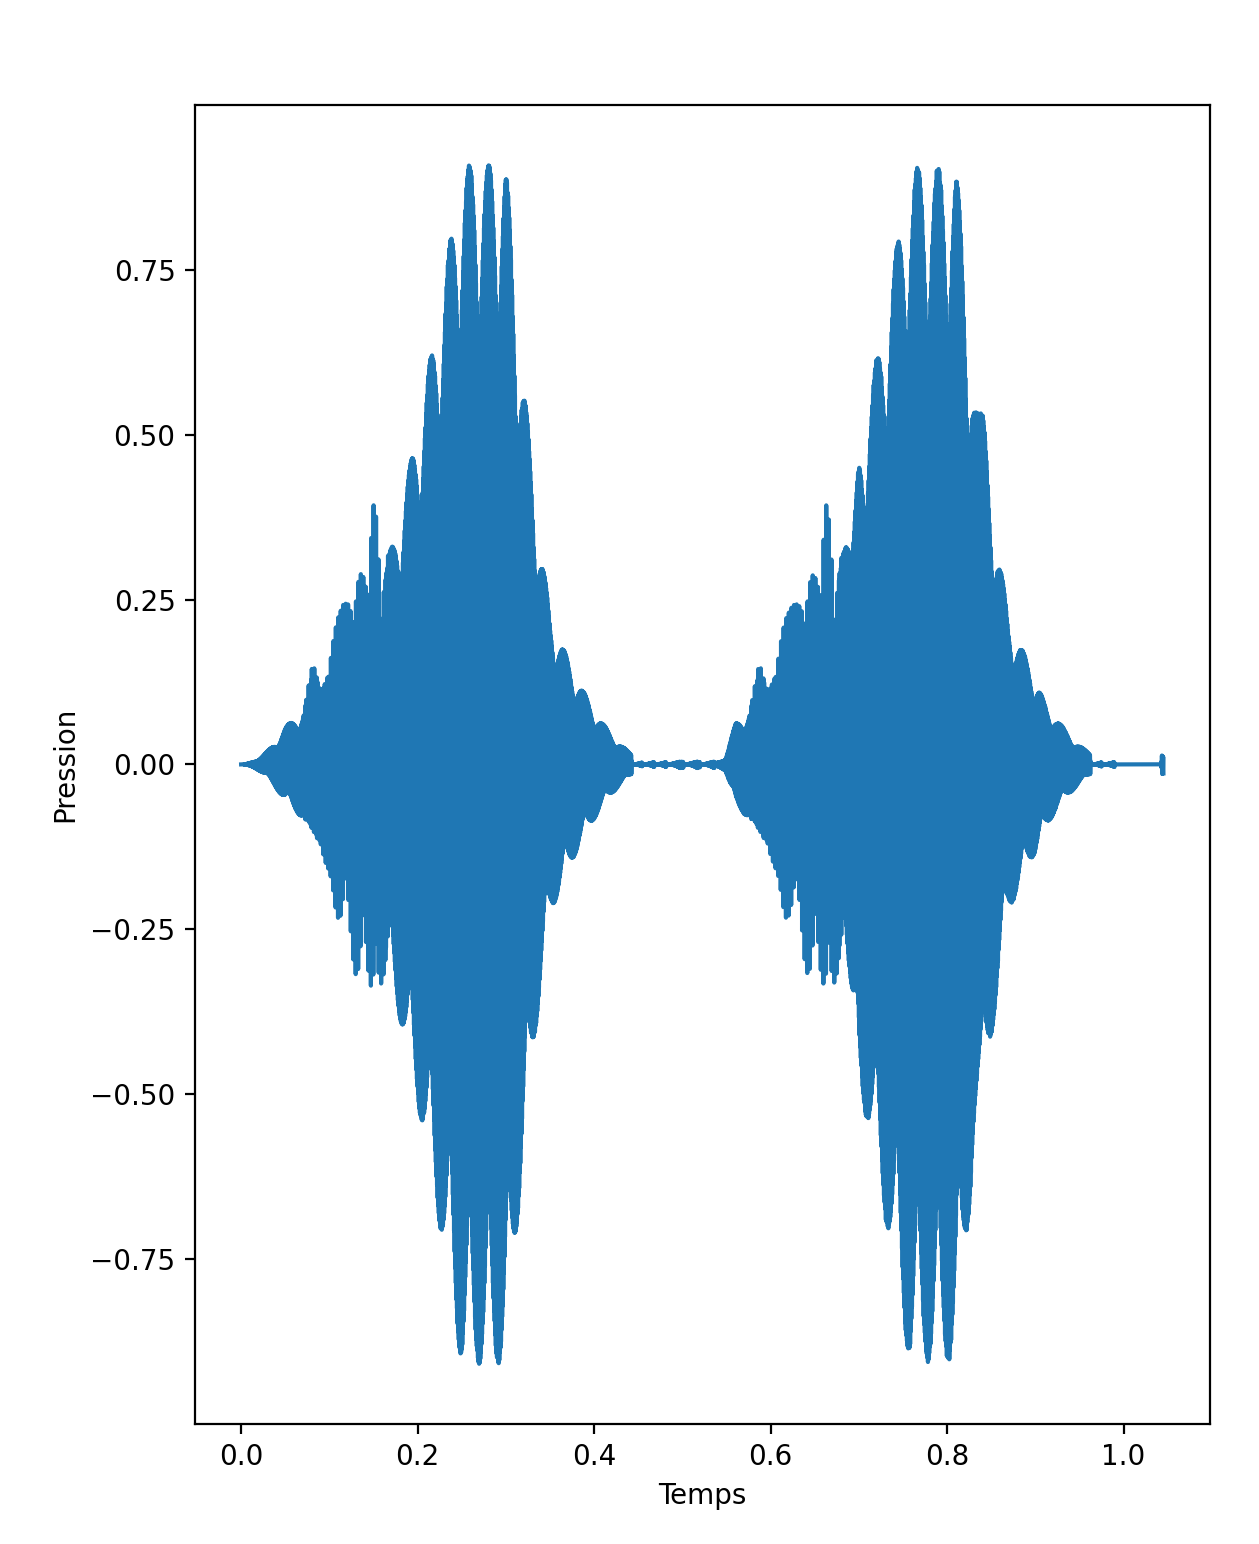
\includegraphics[width=0.5\textwidth]{imgs/sig_sonor.png}
    \caption{Signal temporel du cri de l'aigle}
    \label{fig:eaglesignaltemp}
\end{figure}

\begin{figure}[htbp]
    \centering
    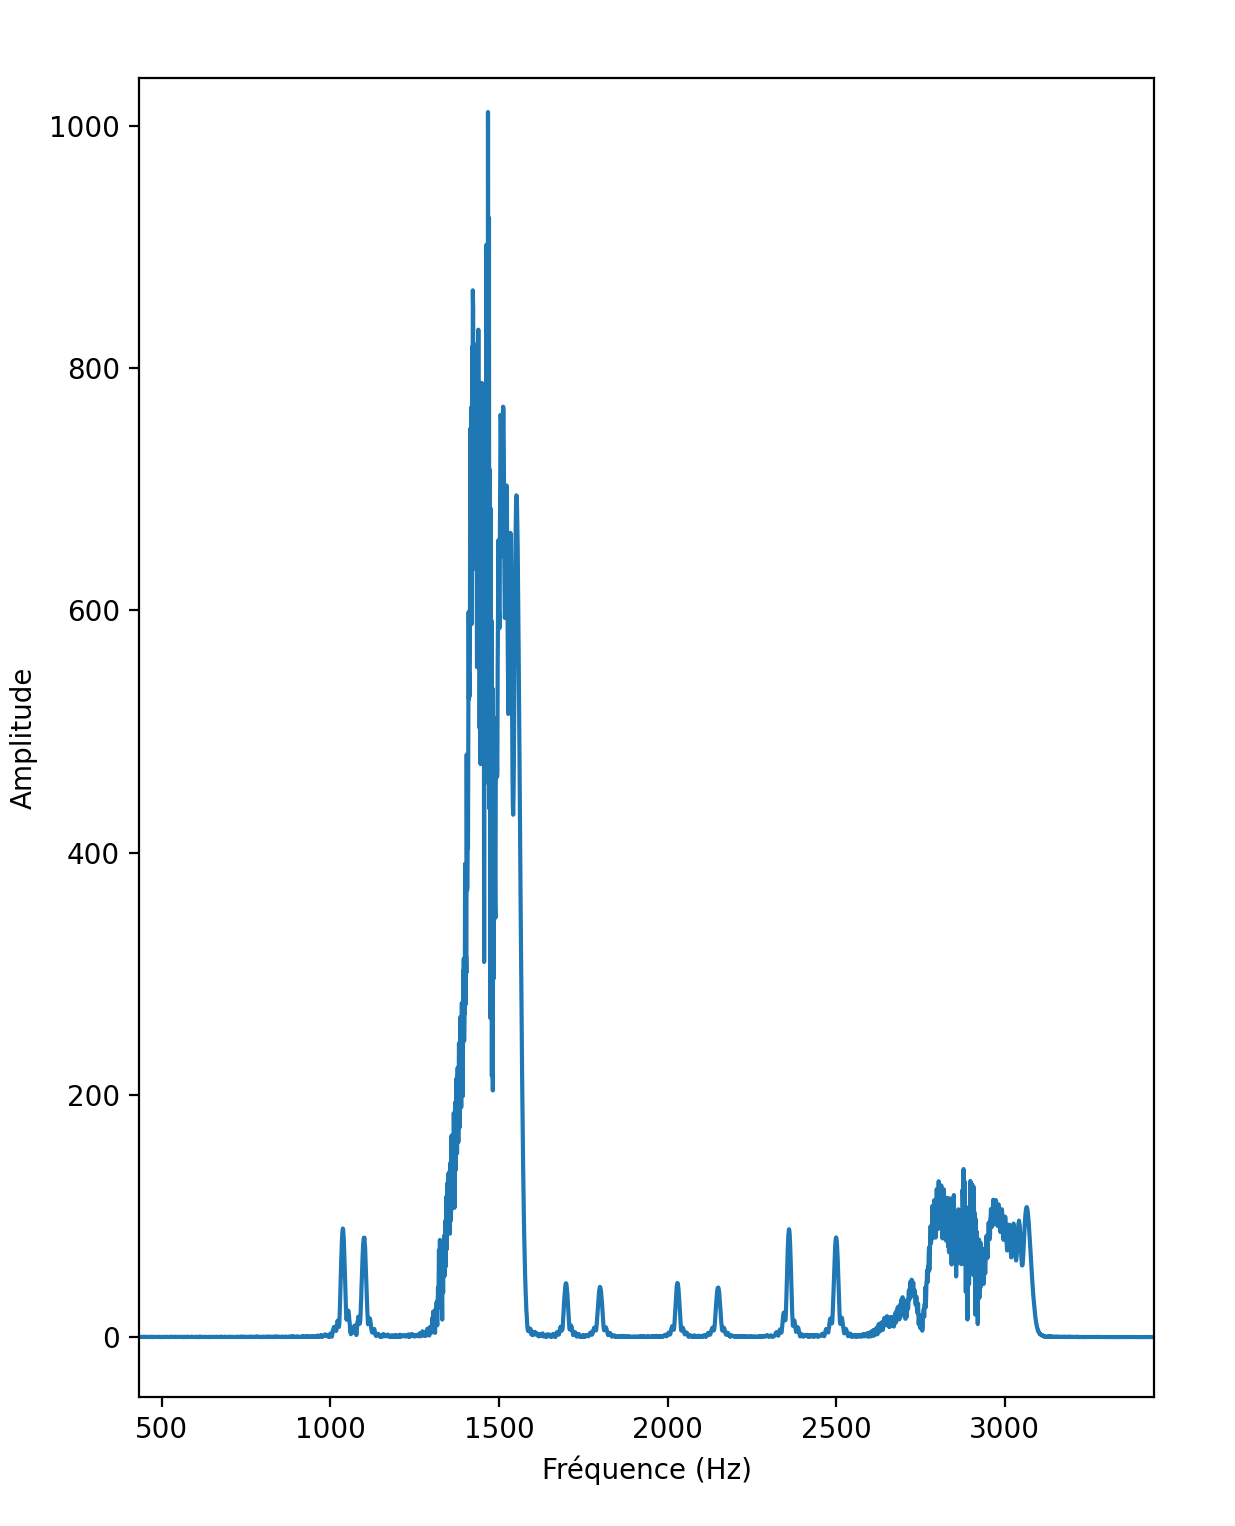
\includegraphics[width=0.5\textwidth]{imgs/fft.png}
    \caption{Transformée de Fourier du cri de l'aigle}
    \label{fig:eaglespectrefreq}
\end{figure}

\begin{figure}[htbp]
    \centering
    \includegraphics[width=0.8\textwidth]{imgs/analyse_temp_freq.eps}
    \caption{Spectrogramme du cri de l'aigle}
    \label{fig:eaglespectrogramme}
\end{figure}

On va utiliser les informations contenues dans ces figures pour synthétiser le cri de l'aigle %
en utilisant un "patron" de fréquences imposé. Pour se faire on va superposer les différentes nappes %
de fréquences visibles sur le Spectrogramme figure \ref{fig:eaglespectrogramme}.

On crée les vecteurs \(s_x\) des différents patrons sur des tronçons de temps. On a juste à additionner %
les différentes harmoniques pour obtenir le son désiré. La fonction \textit{chirp} de scipy.signal qui est la %
même qu'en matlab permet de créer les différentes nappes à chaque tronçon. On peut voir figure %
\ref{fig:eaglespectrogrammesynth} le spectrogramme du son synthétisé.

\begin{figure}
    \centering
    \includegraphics[width=0.8\textwidth]{imgs/spectogramme_synth.eps}
    \caption{Spectrogramme du cri de l'aigle synthétisé}
    \label{fig:eaglespectrogrammesynth}
\end{figure}

Il n'est pas complètement fidèle à l'original et on peut voir des discontinuités (figure \ref{fig:eagle_synth}) %
qui induisent des "poc" dans l'audio.

\begin{figure}
    \centering
    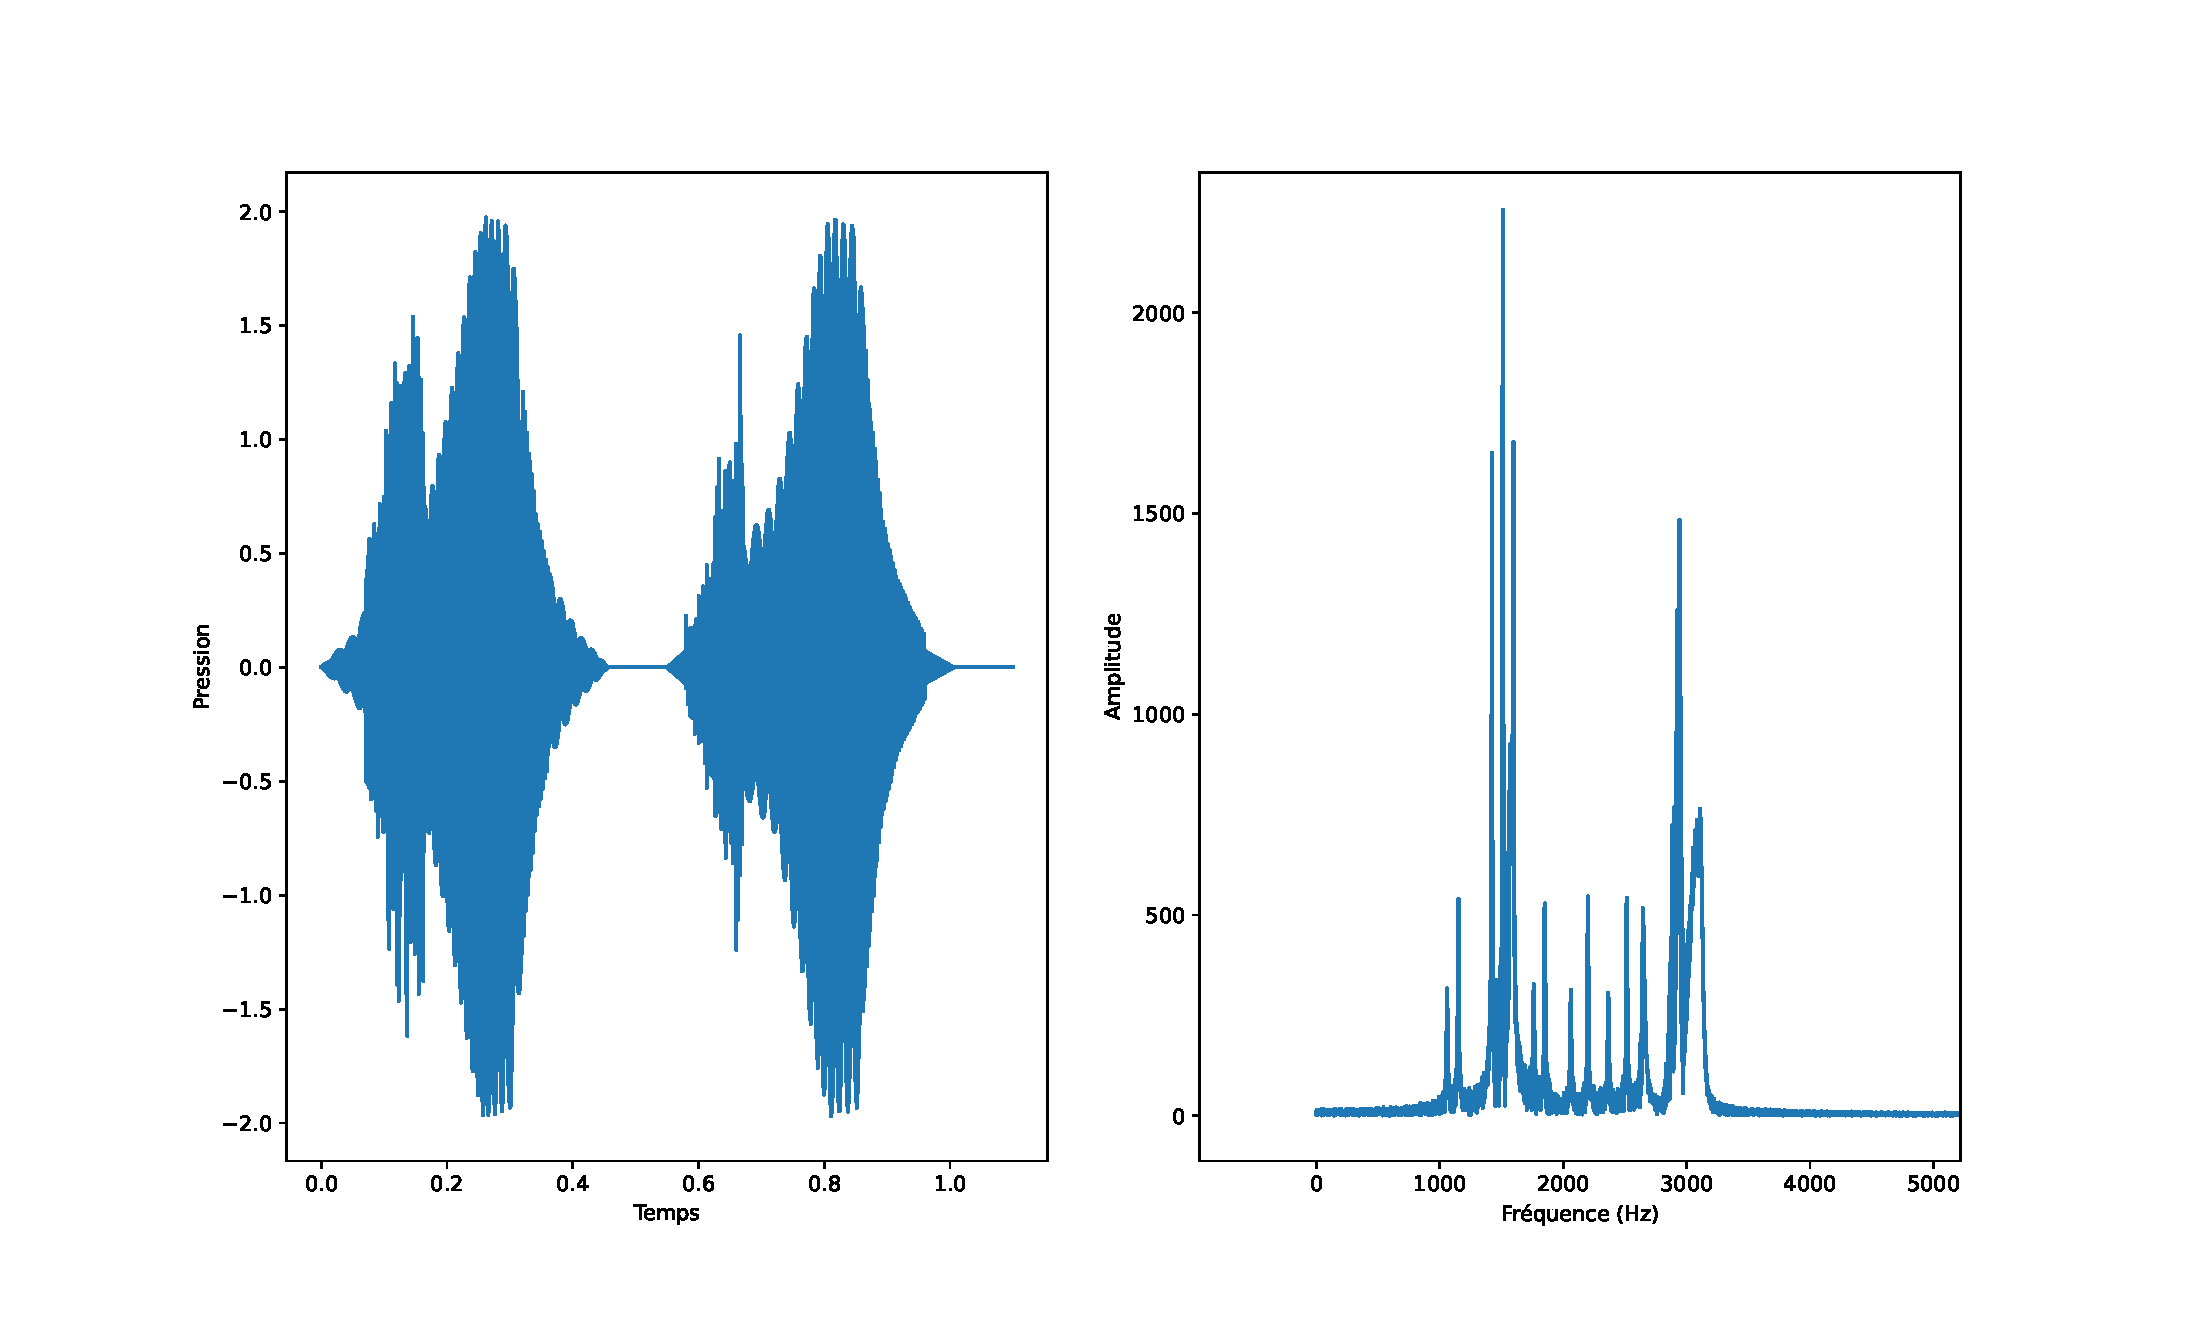
\includegraphics[width=0.8\textwidth]{imgs/synth_eagle.eps}
    \caption{Spectrogramme du cri de l'aigle synthétisé}
    \label{fig:eagle_synth}
\end{figure}

\chapter{Allongement du cri de l'aigle}

Pour étirer la durée du son sans en changer la hauteur, on utilise un facteur d'étirement %
(ici défini à 2) qui double la longueur du signal original. Tout d'abord, on crée un nouveau %
tableau de temps deux fois plus long que celui du signal original. Ensuite, on applique une %
interpolation linéaire pour ajuster le signal à cette nouvelle longueur.

Après cette étape, le son étiré est joué en maintenant la fréquence d'échantillonnage %
d'origine afin de préserver la hauteur du son. Enfin, le son modifié est sauvegardé %
sous l'intitulé \textit{resultat\_stretched.wav} joint au rapport.

\end{document}